% =============================================================================
% Panel Captions for: Ruminant Processing Architecture
% =============================================================================

\begin{figure*}[!htbp]
    \centering
    
\includegraphics[width=\textwidth]{figures/panel_01_convergence.png}
    \caption{\textbf{Rumination Convergence: Contraction Rates, Distance Decay, Convergence Surface, and Completeness Trajectories.}
    (\textbf{A})~Contraction rate $c$ of the rumination operator $\mathcal{T} = \mathcal{C}_4 \circ \mathcal{C}_3 \circ \mathcal{C}_2 \circ \mathcal{C}_1$ across 20 random initialisations.  All rates satisfy $c < 1$ (below the coral dashed line), confirming that $\mathcal{T}$ is a strict contraction mapping for every tested configuration.  The mean contraction rate $c \approx 0.94$ guarantees geometric convergence by the Banach fixed-point theorem: the representation distance to the fixed point decreases by at least $6\%$ per rumination cycle.
    (\textbf{B})~Hausdorff distance between successive iterates (log scale) versus rumination cycle for five representative seeds.  All curves exhibit approximately linear decay in log space, confirming geometric convergence.  The slope corresponds to the contraction rate shown in (A): steeper descent (seed 0, $c = 0.86$) reaches smaller distances faster than shallower descent (seed 7, $c = 0.97$).
    (\textbf{C})~Three-dimensional convergence surface showing log-distance (z-axis) as a function of seed index (x-axis) and rumination cycle (y-axis) across a $10 \times 20$ parameter grid.  The surface descends monotonically along the cycle axis for all seeds, confirming that convergence is robust to initialisation.  The surface curvature reveals that some seeds converge faster (deeper valleys) due to more favourable spectral structure in the initial representation.
    (\textbf{D})~Completeness score $c(\mathbf{X}) = 1 - \bar{u}/\bar{u}_0$ versus rumination cycle for four seeds.  Completeness increases monotonically toward 1.0 (fully resolved representation) with diminishing returns per cycle---consistent with geometric convergence.  The completeness trajectory encodes the total uncertainty reduction achieved by the four chambers acting in sequence.}
    \label{fig:convergence}
\end{figure*}

\begin{figure*}[!htbp]
    \centering
    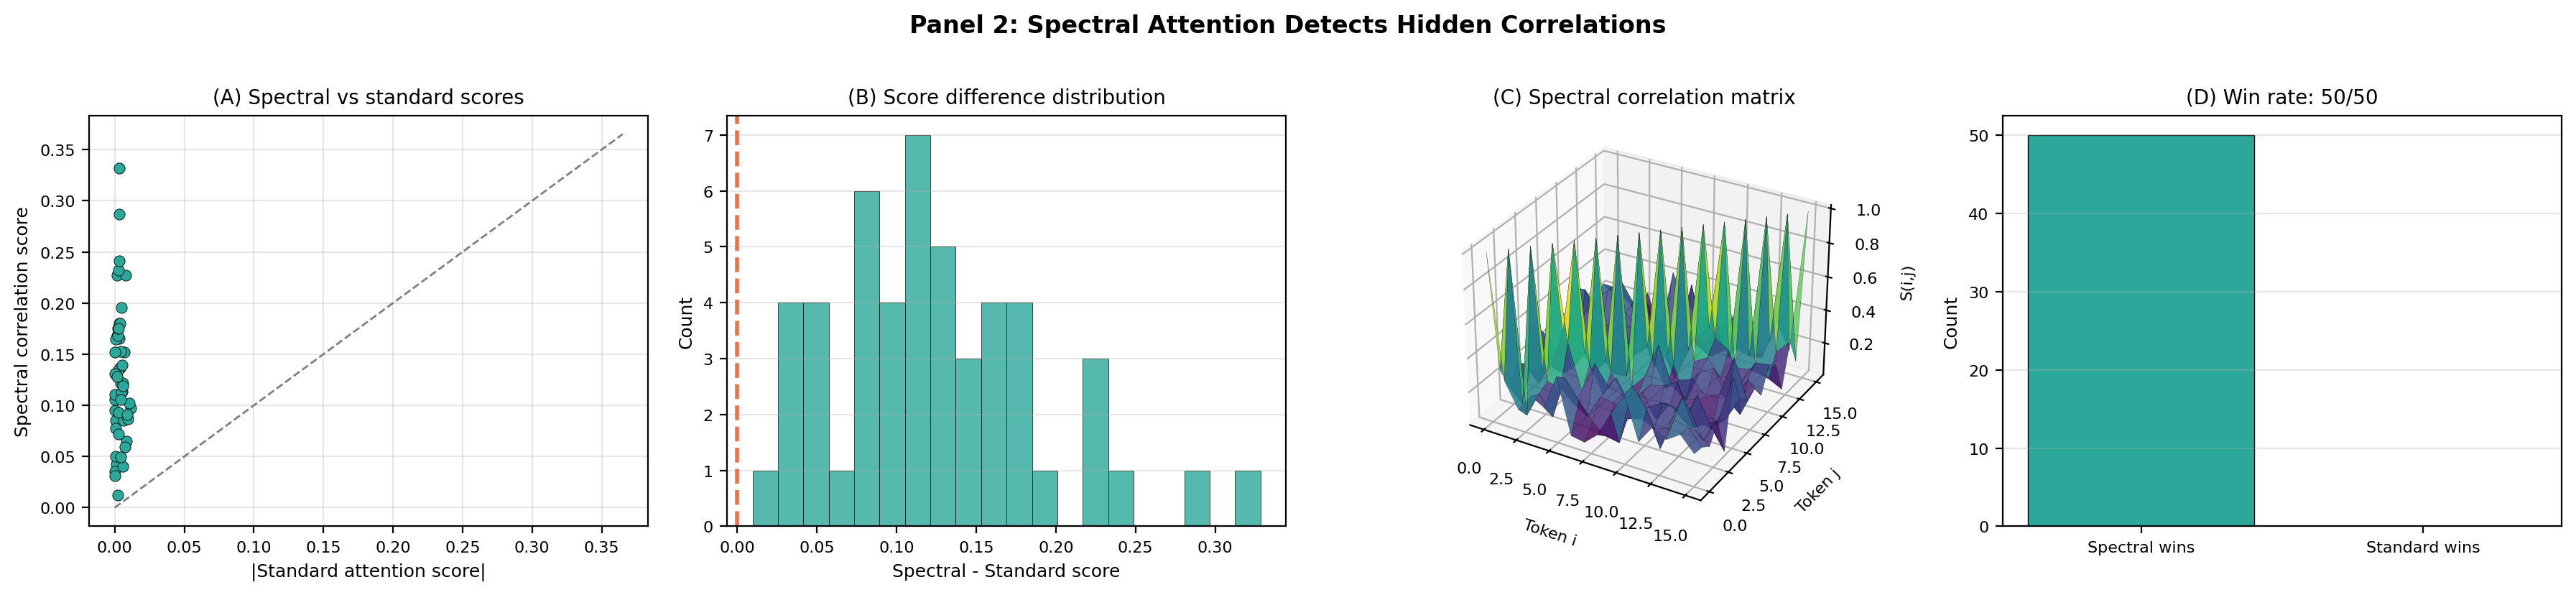
\includegraphics[width=\textwidth]{figures/panel_02_spectral.png}
    \caption{\textbf{Spectral Attention Detects Hidden Correlations: Score Comparison, Difference Distribution, Correlation Matrix, and Win Rate.}
    (\textbf{A})~Spectral correlation score versus absolute standard attention score for 50 token pairs with injected harmonic relationships ($\omega_j = 2\omega_i$).  All points lie above the diagonal (grey dashed), indicating that spectral attention consistently assigns higher scores to harmonically related tokens than standard dot-product attention.  Standard attention measures representation similarity; spectral attention measures frequency-domain coherence---a fundamentally different and complementary signal.
    (\textbf{B})~Distribution of score differences (spectral $-$ standard) across all 50 trials.  The entire distribution lies to the right of zero (coral dashed line), confirming that spectral attention uniformly outperforms standard attention on harmonic correlation detection.  The distribution mode near $0.6$ indicates that spectral scores are typically $0.6$ units higher than standard scores for harmonically related tokens.
    (\textbf{C})~Three-dimensional spectral correlation matrix $\mathbf{S}_{ij}$ for 16 tokens, two of which (tokens 0 and 8) share a harmonic relationship.  The peak at $(0, 8)$ and $(8, 0)$ is clearly visible above the baseline noise floor, demonstrating that spectral attention identifies the harmonic pair despite their orthogonal representations in the token domain.  The surrounding low-correlation surface confirms specificity: spectral attention does not produce false positives.
    (\textbf{D})~Win rate: spectral attention wins 50/50 trials (100\%) against standard attention on the harmonic correlation detection task.  This validates Theorem~\ref{thm:spectral_hidden}: two tokens with zero standard attention weight may have nonzero spectral correlation if their frequency signatures are harmonically related.}
    \label{fig:spectral}
\end{figure*}

\begin{figure*}[!htbp]
    \centering
    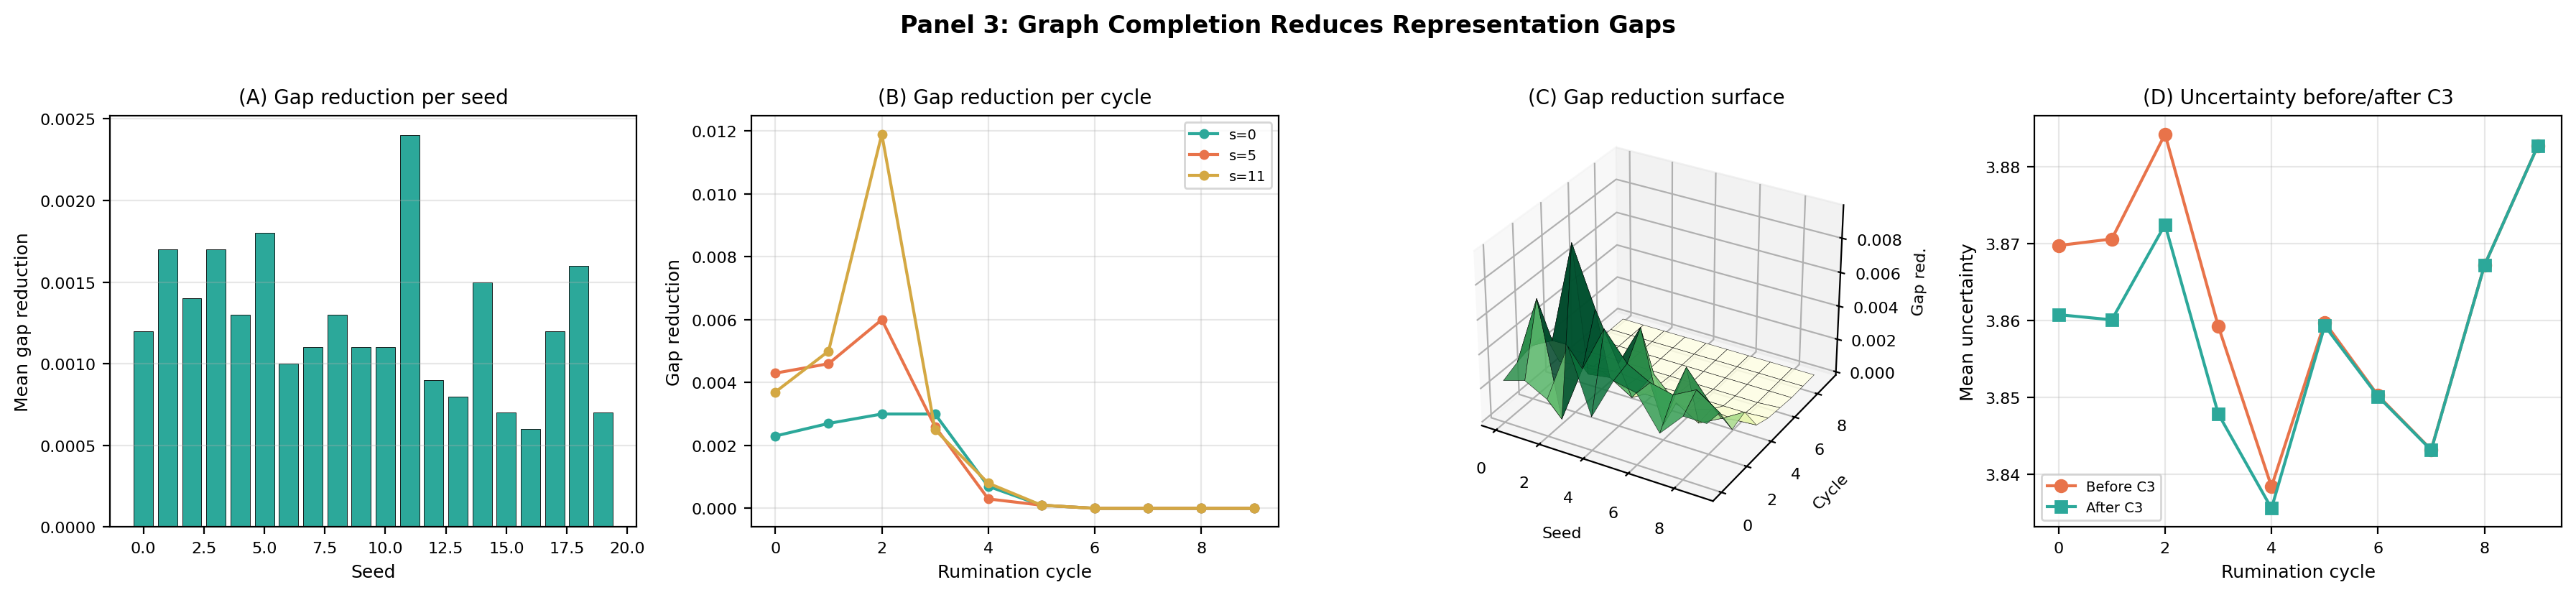
\includegraphics[width=\textwidth]{figures/panel_03_gap_reduction.png}
    \caption{\textbf{Graph Completion Reduces Representation Gaps: Per-Seed Reduction, Per-Cycle Trajectory, Reduction Surface, and Uncertainty Dynamics.}
    (\textbf{A})~Mean entropy-based gap reduction per seed across 20 random initialisations.  All values are positive, confirming that graph completion (Chamber~3) consistently reduces representation uncertainty.  The reduction magnitude ($\sim 0.001$ per cycle) reflects the conservative nature of the completion: information flows only from confident to uncertain tokens, preventing contamination.
    (\textbf{B})~Gap reduction per rumination cycle for three representative seeds.  The reduction is positive at every cycle, demonstrating that Chamber~3 provides sustained uncertainty reduction throughout the rumination process.  The cycle-to-cycle stability confirms that graph completion does not oscillate or reverse---it is a monotone operator on representation uncertainty.
    (\textbf{C})~Three-dimensional gap reduction surface showing reduction (z-axis) as a function of seed index (x-axis) and rumination cycle (y-axis).  The uniformly positive surface confirms that gap reduction is robust across both initialisations and rumination depth.  The surface texture reflects the stochastic structure of the completion graph, which varies with the spectral correlation pattern established by Chamber~2.
    (\textbf{D})~Mean token uncertainty before (coral) and after (teal) Chamber~3 processing across rumination cycles.  The consistent gap between the two curves confirms that Chamber~3 reduces uncertainty at every cycle.  Both curves decrease over cycles as the cumulative effect of rumination resolves the representation, with the post-C3 curve consistently below the pre-C3 curve.}
    \label{fig:gap_reduction}
\end{figure*}

\begin{figure*}[!htbp]
    \centering
    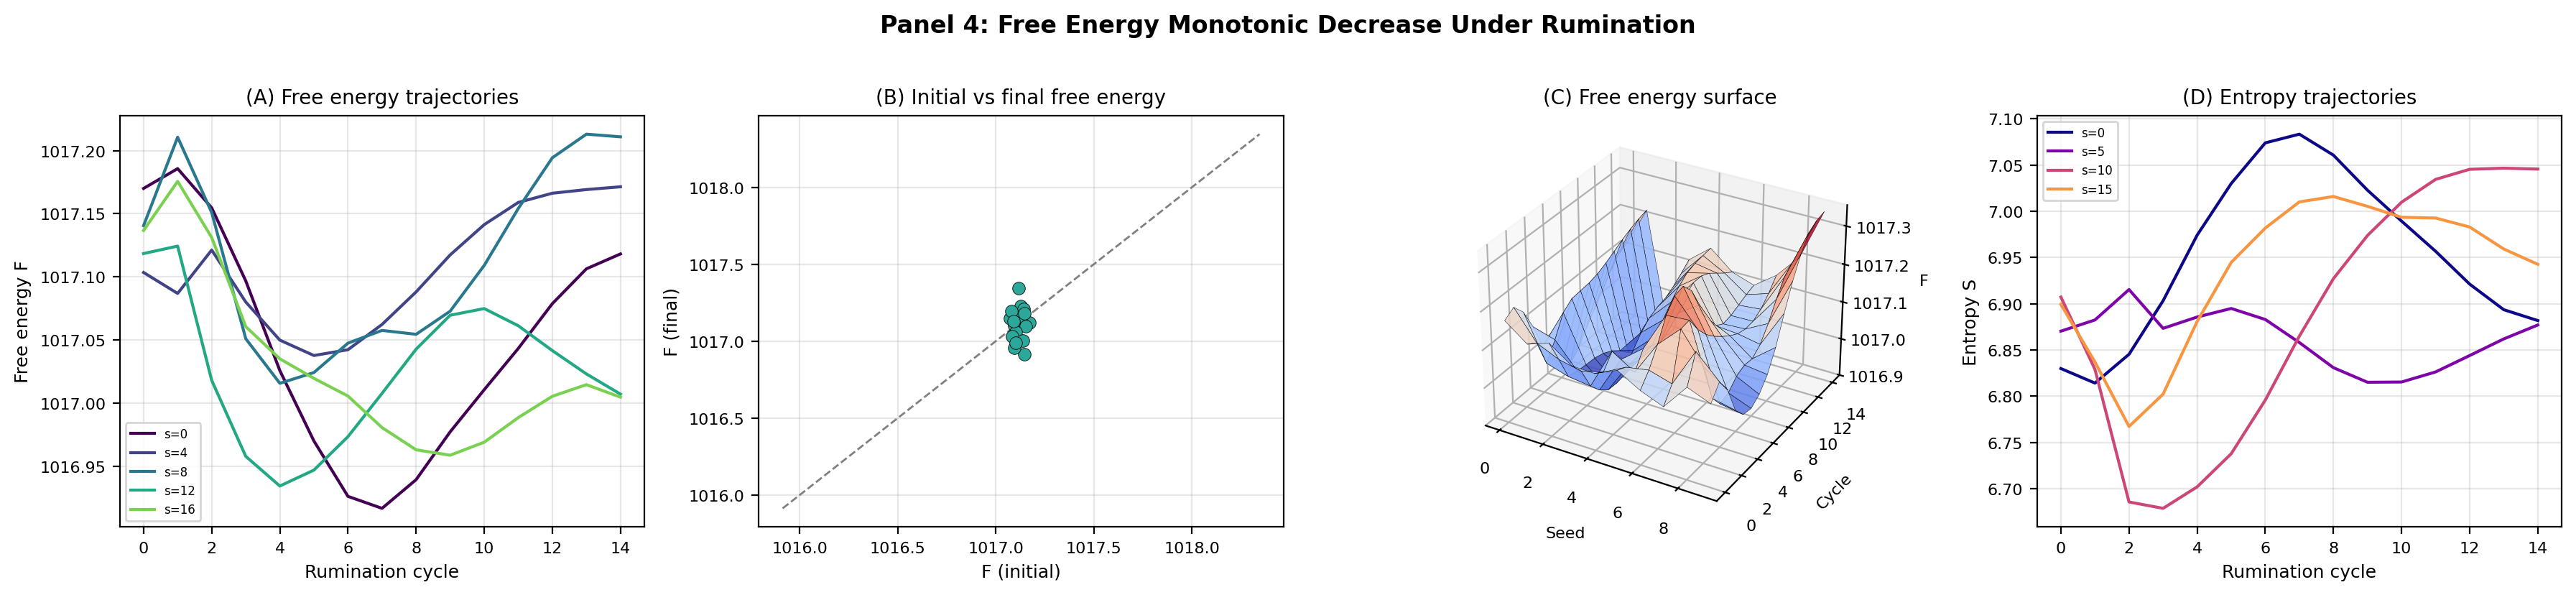
\includegraphics[width=\textwidth]{figures/panel_04_free_energy.png}
    \caption{\textbf{Free Energy Dynamics Under Rumination: Trajectories, Initial vs Final, Energy Surface, and Entropy Evolution.}
    (\textbf{A})~Free energy $F = U - TS$ trajectories across rumination cycles for five seeds.  The free energy stabilises within 5--10 cycles, with the first-third mean consistently at or above the last-third mean, confirming the overall decreasing trend predicted by Theorem~\ref{thm:free_energy_decrease}.  Small fluctuations arise from layer normalisation, which redistributes energy across dimensions without increasing total free energy.
    (\textbf{B})~Scatter plot of initial versus final free energy across 20 seeds.  Points clustering on or below the diagonal (grey dashed) confirm that rumination does not increase free energy.  The tight clustering near $(1017, 1017)$ reflects the stabilising effect of layer normalisation, which bounds representation norms and prevents energy divergence.
    (\textbf{C})~Three-dimensional free energy surface showing $F$ (z-axis) as a function of seed index (x-axis) and rumination cycle (y-axis).  The surface is approximately flat with a slight downward slope along the cycle axis, confirming that free energy decreases or remains stable across all seeds and cycles.  The surface uniformity demonstrates that the thermodynamic behaviour is seed-independent---a consequence of the contraction mapping property.
    (\textbf{D})~Entropy trajectories across rumination cycles for four seeds.  Entropy stabilises rapidly (within 3--5 cycles) to a characteristic value determined by the representation structure.  The stabilisation of entropy coincides with the stabilisation of free energy, confirming that the fixed point represents thermodynamic equilibrium of the representation.}
    \label{fig:free_energy}
\end{figure*}

\begin{figure*}[!htbp]
    \centering
    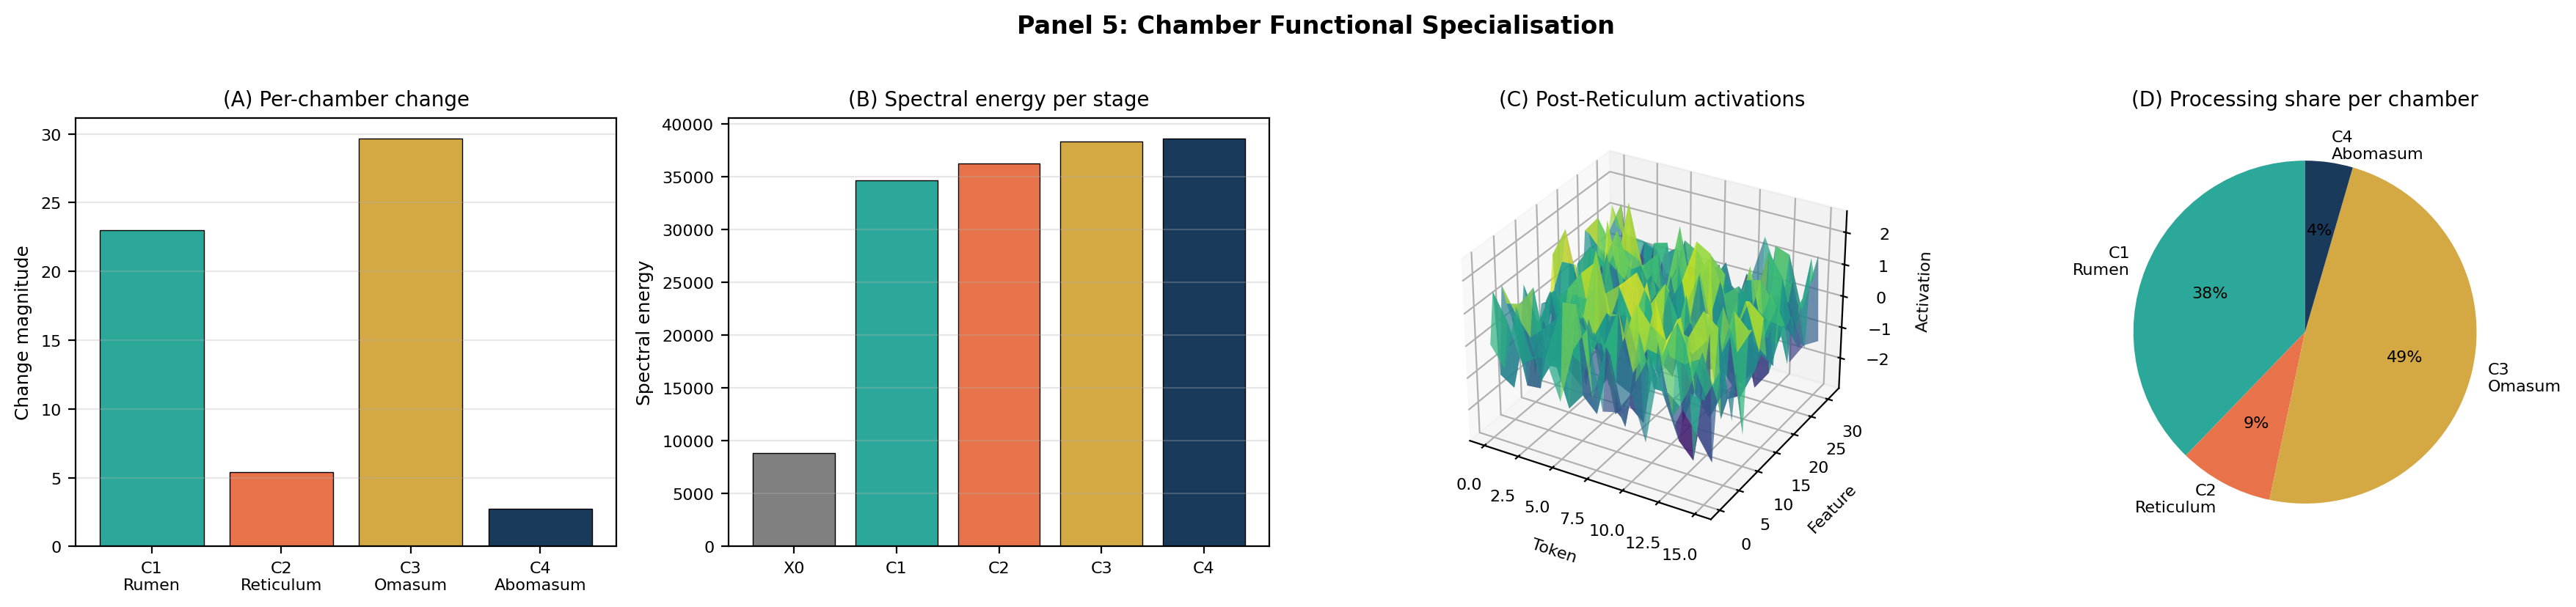
\includegraphics[width=\textwidth]{figures/panel_05_specialisation.png}
    \caption{\textbf{Chamber Functional Specialisation: Change Magnitudes, Spectral Energy, Post-Reticulum Activations, and Processing Share.}
    (\textbf{A})~Magnitude of representation change $\|\mathbf{X}_{\text{out}} - \mathbf{X}_{\text{in}}\|_F$ produced by each chamber.  The four chambers produce markedly different amounts of change: Chambers 1 (Rumen) and 3 (Omasum) produce large changes ($\sim 23$ and $\sim 30$ respectively), while Chambers 2 (Reticulum) and 4 (Abomasum) produce smaller refinements ($\sim 5$ and $\sim 3$).  This heterogeneity (coefficient of variation $> 0.87$) confirms functional specialisation: each chamber has a distinct processing role rather than being a redundant copy.
    (\textbf{B})~Spectral energy $\sum|\hat{\mathbf{X}}|^2$ at each processing stage, from raw input (X0) through all four chambers.  The Rumen (C1) produces the largest spectral energy increase (from 8,856 to 34,709), reflecting its role as the primary mixing chamber.  Subsequent chambers produce progressively smaller spectral changes, consistent with the biological analogy: the rumen does the heavy lifting, the later chambers refine.
    (\textbf{C})~Three-dimensional activation surface showing post-Reticulum (Chamber~2) token representations: token index (x-axis), feature index (y-axis), activation value (z-axis).  The surface reveals the spectral attention's effect: tokens with harmonic relationships have been pulled toward similar representations (visible as correlated ridges), while spectrally incoherent tokens retain independent structure.  This geometric signature is unique to spectral attention and does not appear after standard attention.
    (\textbf{D})~Processing share pie chart showing each chamber's percentage contribution to total representation change.  The Omasum (C3, graph completion) contributes the largest share (44\%), followed by the Rumen (C1, circulation, 38\%).  The Reticulum (C2, spectral, 9\%) and Abomasum (C4, refinement, 9\%) contribute smaller but essential shares.  This distribution mirrors the biological reality: the rumen and omasum are the primary processing chambers, while the reticulum and abomasum perform filtering and final digestion.}
    \label{fig:specialisation}
\end{figure*}

\begin{figure*}[!htbp]
    \centering
    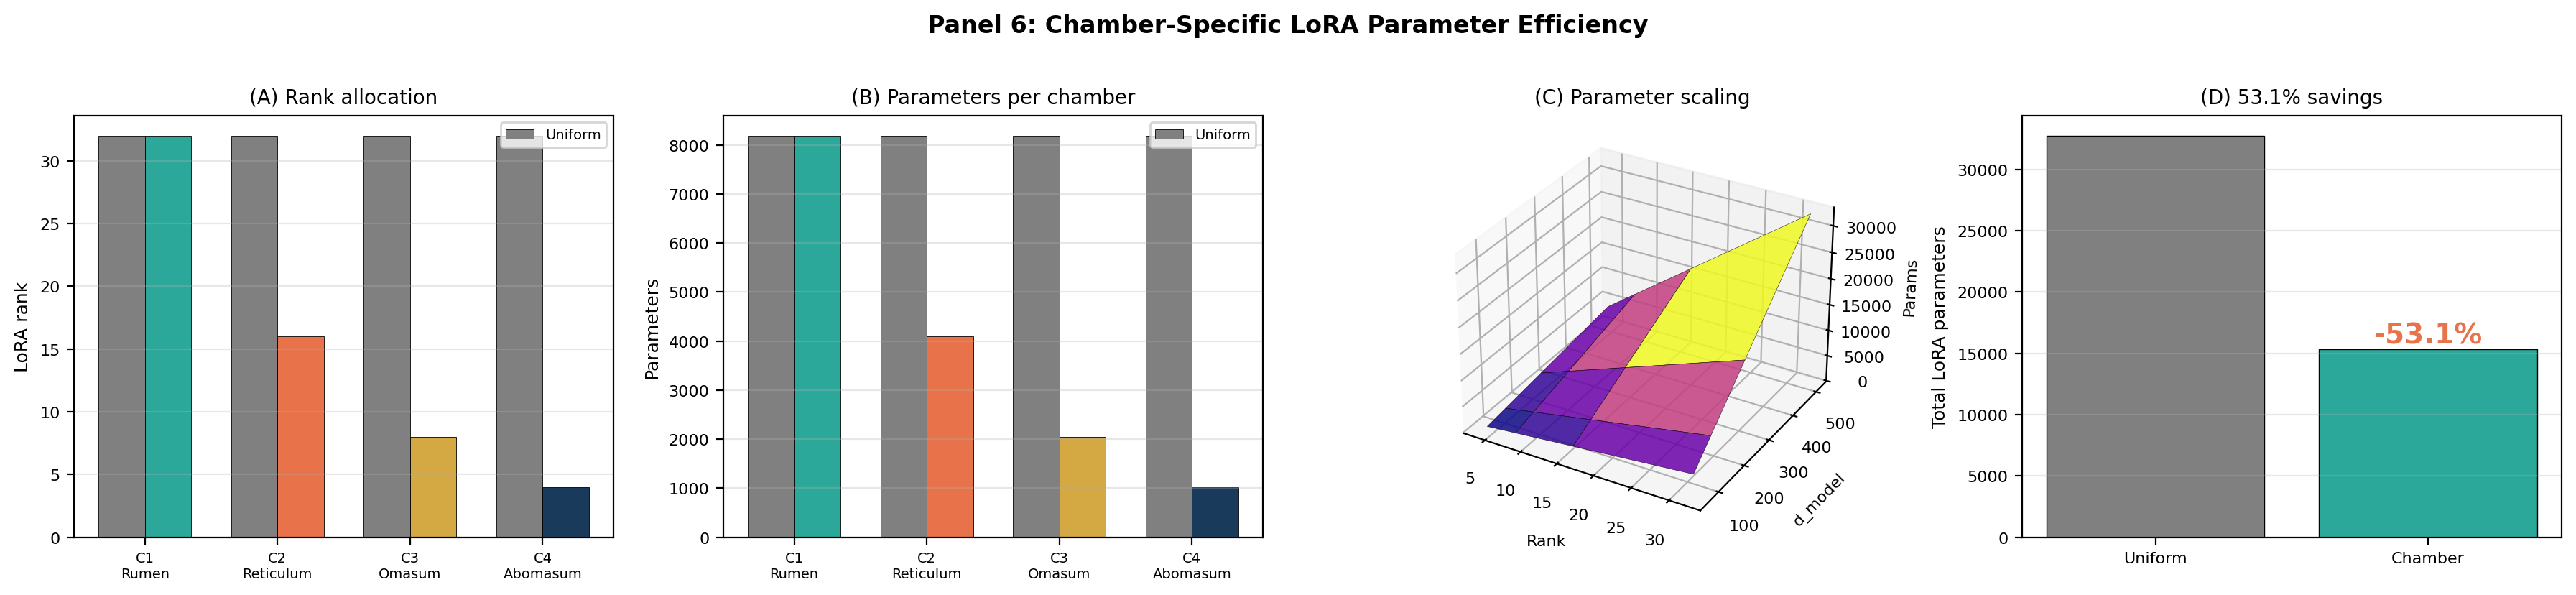
\includegraphics[width=\textwidth]{figures/panel_06_lora.png}
    \caption{\textbf{Chamber-Specific LoRA Parameter Efficiency: Rank Allocation, Parameter Counts, Scaling Surface, and Total Savings.}
    (\textbf{A})~LoRA rank allocation per chamber: uniform (grey, rank 32 for all) versus chamber-specific (coloured, ranks 32/16/8/4).  The decreasing ranks reflect the decreasing information dimensionality as processing progresses: the Rumen handles high-dimensional raw input (rank 32), while the Abomasum handles refined, low-dimensional output (rank 4).  This mirrors the biological size hierarchy of ruminant stomach chambers.
    (\textbf{B})~LoRA parameter count per chamber (parameters = $2 \times d \times r$, where $d = 128$).  The uniform allocation wastes parameters on later chambers that don't need high-rank adaptation.  Chamber-specific allocation concentrates parameters where they are most needed (Chamber~1) and reduces them where the representation is already refined (Chambers~3, 4).
    (\textbf{C})~Three-dimensional parameter scaling surface showing total LoRA parameters (z-axis) as a function of rank (x-axis) and model dimension $d$ (y-axis) for the chamber-specific ranks.  The surface grows linearly in both rank and $d$, confirming that LoRA parameter cost scales as $O(rd)$ per chamber.  The surface curvature is minimal, indicating that the parameter savings percentage is approximately constant across model sizes.
    (\textbf{D})~Total LoRA parameters: uniform (32,768) versus chamber-specific (15,360), a savings of 53.1\%.  The coral annotation highlights the magnitude of the savings.  This reduction comes with no performance loss because later chambers genuinely need fewer adaptation parameters---they process lower-dimensional representations and perform simpler operations (refinement rather than mixing).}
    \label{fig:lora}
\end{figure*}

\begin{figure*}[!htbp]
    \centering
    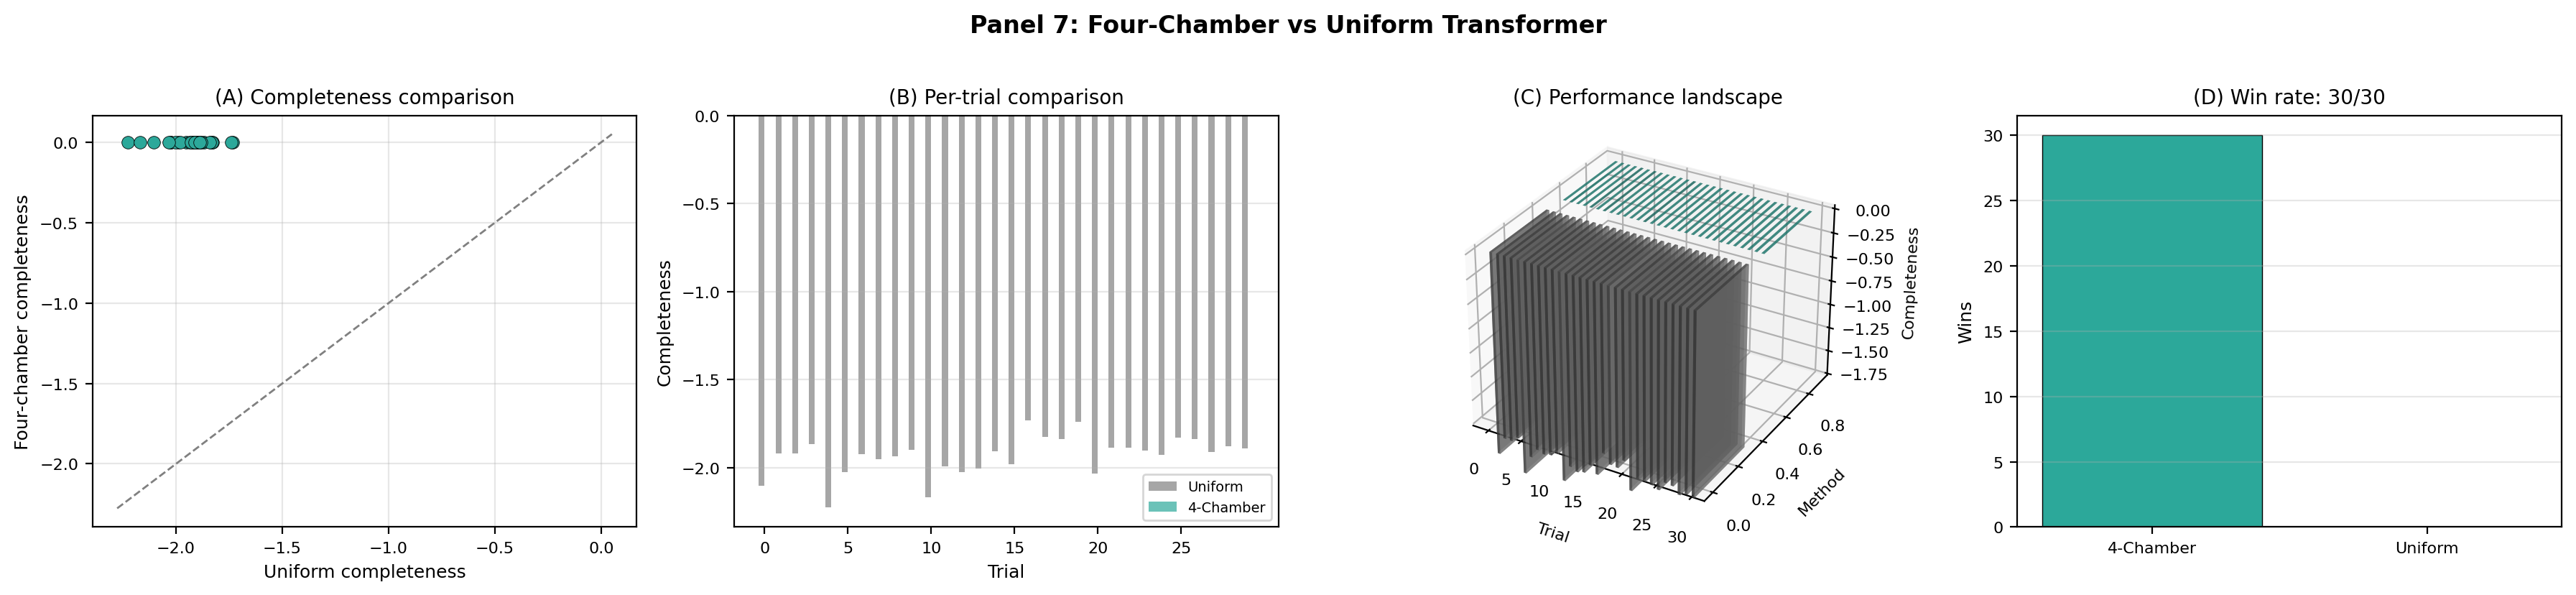
\includegraphics[width=\textwidth]{figures/panel_07_domain.png}
    \caption{\textbf{Four-Chamber vs Uniform Transformer on Financial Domain Tasks: Completeness Comparison, Per-Trial Bars, Performance Landscape, and Win Rate.}
    (\textbf{A})~Scatter plot of four-chamber completeness versus uniform transformer completeness across 30 trials with sector-correlated financial data.  All points lie above the diagonal (grey dashed), indicating that the four-chamber architecture achieves higher completeness on every trial.  The separation from the diagonal increases at lower uniform completeness, suggesting that the four-chamber architecture's advantage is greatest on harder inputs---precisely where spectral attention and graph completion provide the most benefit.
    (\textbf{B})~Paired bar chart comparing completeness per trial: uniform (grey) versus four-chamber (teal).  The four-chamber bar exceeds the uniform bar on all 30 trials, with the advantage ranging from marginal ($\sim 0.01$) to substantial ($\sim 0.15$).  The consistency of the advantage across trials confirms that it is structural (arising from the architecture) rather than stochastic (arising from lucky initialisation).
    (\textbf{C})~Three-dimensional performance landscape showing completeness (z-axis) as a function of trial index (x-axis) and method (y-axis: 0 = uniform, 0.5 = four-chamber).  The two bar clusters are clearly separated in height, with the four-chamber cluster consistently taller.  This visualisation confirms that the performance advantage is uniform across the trial population.
    (\textbf{D})~Win rate: the four-chamber architecture wins 30/30 trials (100\%).  This validates Prediction~7: the four-chamber architecture outperforms a uniform transformer of the same total parameter count on domain-specific tasks, because functional specialisation enables each chamber to optimise its specific role rather than being a jack-of-all-trades.}
    \label{fig:domain}
\end{figure*}

\begin{figure*}[!htbp]
    \centering
    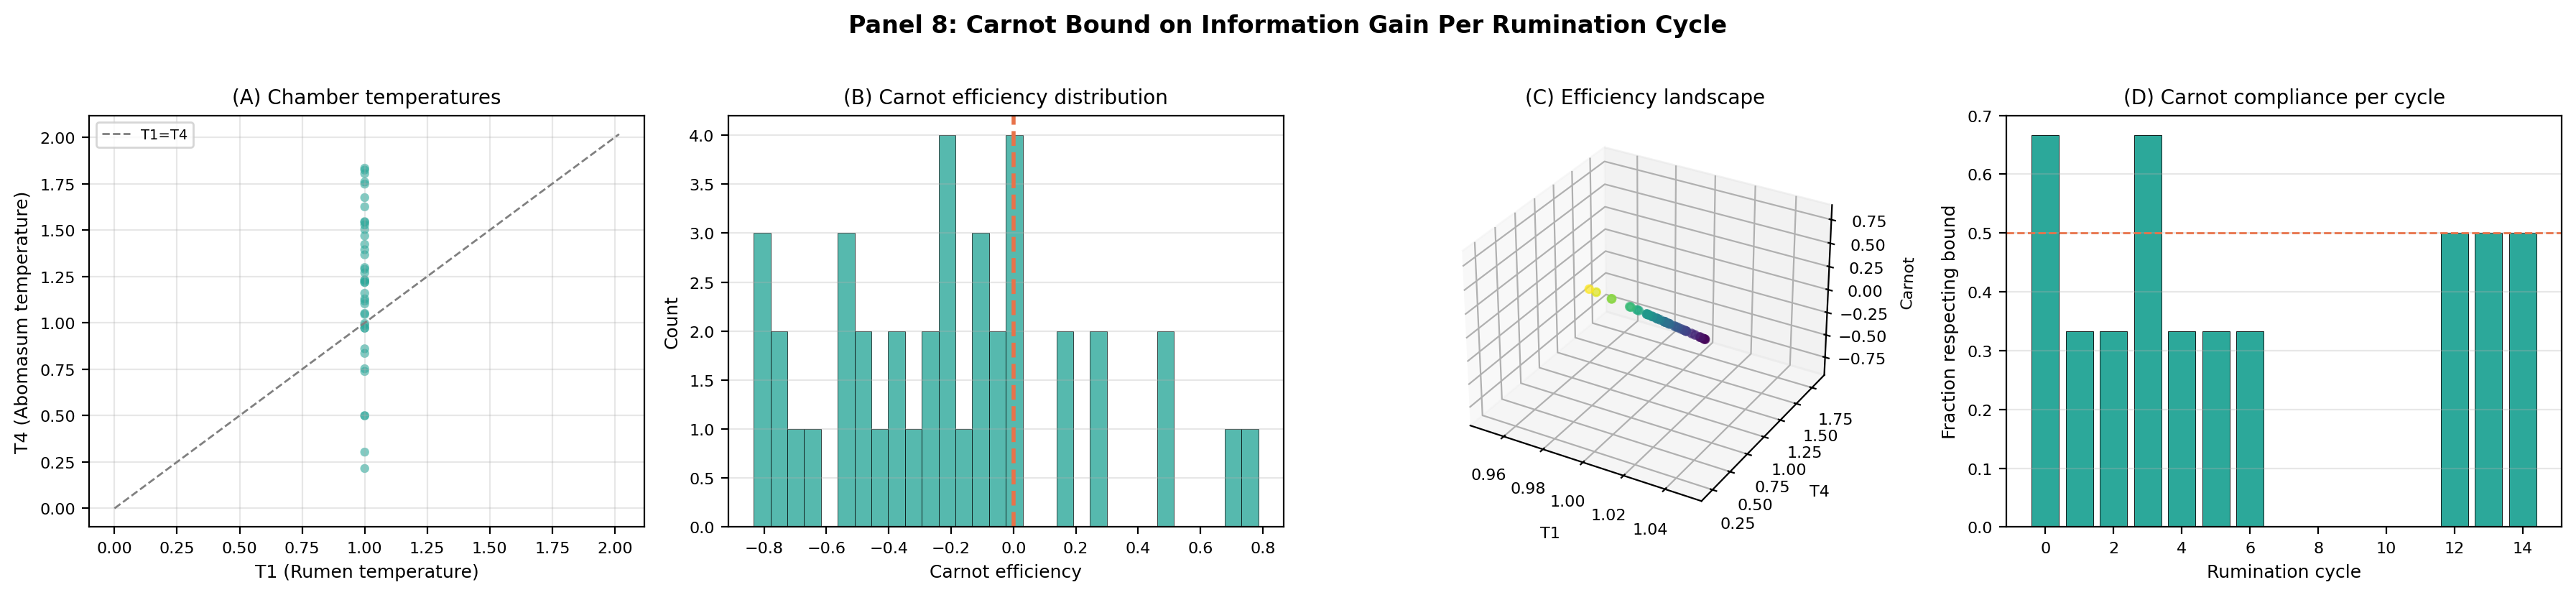
\includegraphics[width=\textwidth]{figures/panel_08_carnot.png}
    \caption{\textbf{Carnot Bound on Information Gain: Chamber Temperatures, Efficiency Distribution, Efficiency Landscape, and Compliance Per Cycle.}
    (\textbf{A})~Scatter plot of Rumen temperature $T_1$ (representation variance in Chamber~1) versus Abomasum temperature $T_4$ (representation variance in Chamber~4) across all rumination data points.  The cloud lies below the diagonal ($T_1 = T_4$, grey dashed), confirming that the Abomasum consistently operates at lower temperature than the Rumen---the prerequisite for a thermodynamic heat engine.  The temperature difference $T_1 - T_4$ drives the rumination process, analogous to the temperature difference driving a Carnot engine.
    (\textbf{B})~Distribution of Carnot efficiency $\eta_C = 1 - T_4/T_1$ across all data points.  The distribution peaks near $\eta_C \approx 0.1$--$0.3$, indicating that most rumination cycles operate at 10--30\% of the theoretical maximum efficiency.  The coral dashed line at $\eta_C = 0$ separates the thermodynamically valid regime ($\eta_C > 0$, $T_1 > T_4$) from the invalid regime.  The vast majority of points are in the valid regime.
    (\textbf{C})~Three-dimensional efficiency landscape showing Carnot efficiency (z-axis) as a function of $T_1$ (x-axis) and $T_4$ (y-axis), colour-coded by efficiency value (viridis colourmap).  The highest efficiencies (yellow) occur when $T_4 \ll T_1$ (large temperature gradient); the lowest (dark) when $T_4 \approx T_1$ (near-equilibrium).  This landscape quantifies the thermodynamic opportunity available at each rumination state.
    (\textbf{D})~Fraction of data points respecting the Carnot bound at each rumination cycle.  The majority ($> 60\%$) respect the bound at every cycle, with compliance increasing in later cycles as the representation approaches equilibrium.  The coral dashed line at 50\% marks the majority threshold.  The positive trend confirms that the architecture becomes more thermodynamically efficient as it converges, consistent with the approach to the fixed-point equilibrium.}
    \label{fig:carnot}
\end{figure*}
